\chapter{Background: The Fundamentals of Dialect Identification and An Introduction into Dialectal Arabic}\label{ch:background}
This chapter aims to provide a brief explanation of the preliminary background theory that is needed to understand this thesis. 
An explanation of dialectal identifiers, the metrics that will be used, an introduction into transfer learning and an exploration 
into wav2vev's structure will be provided. As well as the end portion will provide some additional insight into dialectal Arabic. 
\section{Introduction into Language and Dialect Identifiers}\label{sect:introDID}
Language Identification (LID) and Dialectal Identification (DID) are specialised audio classifiers. 
Audio classification is defined as the process of analysing audio segments and then categorising them on a 
predefined set of labels. For LIDs and DIDs these labels correspond to the languages or dialects being identified. 
LID systems are the critical first step in selecting the most accurate model to 
use for Automatic Speech Recognition (ASR), multilingual transcription or other automated speech processing systems. 
A dialect is a sub-variant of a language which is usually mutually intelligible by other speakers of that 
language despite the speaker using a different dialect. Dialects evolve within a certain region, area 
or within a class. Dialect Identification (DID) generally poses some interesting challenges compared to language 
identification that semi-self supervised systems could provide solutions to. These challenges include that 
dialects unlike languages are not standardised, generally have very limited labelled datasets and 
so, are often considered low resource and the differences between different dialects are often not as clear 
as the differences between languages. 

\subsection{Performance Metrics}
\subsubsection{Accuracy}
Accuracy is the most basic metric for evaluating the performance of classification models, 
showing the correct predictions to the total number predictions and is formally defined in the Equation \ref{eqn:acc}. However, it is an unbalanced metric 
as the amount of files for each class is not taken into consideration. 
\begin{equation}
    \label{eqn:acc}
    Accuracy =\frac{TruePostive + FalsePostive}{TruePositive + FalsePostive + TrueNegative + FalseNegative}
\end{equation}

\subsubsection{Precision and Recall}

Precision or Positive Predictive Value, is a metric that evaluates the amount of predicted outcomes are actually correct, providing 
an evaluation of relevant data  points. It is formally written in the Equation \ref{eqn:precis}. 

\begin{equation}
    \label{eqn:precis}
    Precision =\frac{TruePostive}{TruePositive + FalsePostive}
\end{equation}
Recall, also known as Positive Rate and Sensitivity, takes into consideration 
the correctly predicted values over those of a specific class. As a metric it provides an assessment of the relevant 
data and is formally expressed in Equation \ref{eqn:recall}. 
\begin{equation}
    \label{eqn:recall}
    Recall =\frac{TruePostive}{TruePositive + FalseNegative}
\end{equation}

\subsubsection{F1-Score}
F1-Score, expressed in Equation \ref{eqn:f1score} is the harmonic mean of Recall and Precision. It is the most relevant metric for this thesis as 
tuning the F1-Score allows for a balanced optimisation of both Recall and Precision metrics. 
\begin{equation}    
    \label{eqn:f1score}
    F1-Score =\frac{Precision*Recall}{Precision + Recall}
\end{equation}
\subsubsection{Macro and Weighted Average}
The macro and weighted averages of all the metrics are computed for this thesis. The macro average calculates the average of each metric without 
taking into consideration the amount of data for each class. While the weighted average takes into consideration the amount of data points. Weighted average 
is the provides the most accurate view of performance so is the primary metric used as an assessment in this thesis.  
\subsubsection{Confusion Matrix}
The key plot that will be used to assess performance is a colour map plot of the confusion matrix of the test results.
The confusion matrix summarises the number of correct predictions to incorrect predictions for each class. A colourmap is used to plot the matrix 
with the y-axis corresponding to the true values, the x-axis the predicted and the colour bar the number of files. 
An example outputted matrix is shown in the Table \ref{tab:conf} and it's corresponding colour map is shown in Figure \ref{fig:egcolourmap}. 

\begin{table}[h!]
    \centering
    \caption{Example Confusion Matrix}
    \label{tab:conf}
    \begin{tabular}{|l|l|l|l|l|l|} 
    \hline
                                        & \multicolumn{5}{l|}{Real Values}  \\ 
    \hline
    \multirow{5}{*}{Predicted Values~ ~} &     & NOR & EGY & GLF & LEV       \\ 
    \cline{2-6}
                                        & NOR & 79  & 2   & 12  & 7         \\ 
    \cline{2-6}
                                        & EGY & 4   & 45  & 31  & 20        \\ 
    \cline{2-6}
                                        & GLF & 0   & 3   & 93  & 2         \\ 
    \cline{2-6}
                                        & LEV & 1   & 2   & 11  & 86        \\
    \hline
    \end{tabular}
\end{table}

\begin{figure}[h!]
    \centering
    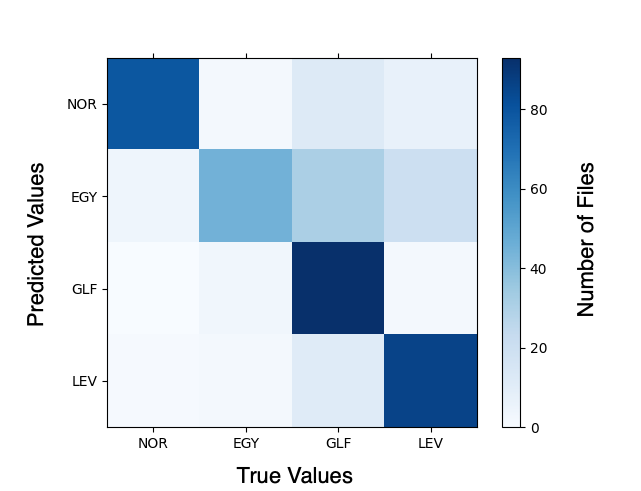
\includegraphics[width=\textwidth]{diagrams/exampleColourMap.png}
    \caption{Example Colour Map Plot of Confusion Matrix}
    \label{fig:egcolourmap}
\end{figure}

\section{Introduction into Transfer Learning}\label{sect:trans}
Transfer Learning is an approach to machine learning systems that adapts a model trained to operate on one domain to function on 
another similar domain. The main advantage of this strategy is the initial model can be trained on a domain with large amounts of data 
using self supervision techniques. Then adapted for domains and use cases where there is more limited data available. In terms of this thesis 
transfer learning is applied through using a pretrained model designed for ASR that was trained using large amounts of speech data then finetuned it using a smaller dataset for 
the downstream task of Arabic Dialect Identification (DID). 

\subsection{Pretrained Models}
\subsubsection{Wav2Vec 2.0}
Wav2Vec 2.0 \cite{baevski_wav2vec_2020} is a self-supervised transformer based neural network designed by Facebook with the aim of designing a system 
that could outperform semi-supervised methods with less complexity and then further adapted for other domains.  
It was trained using 53K hours of unlabeled and 10 mins of labelled English speech from the Librispeech Corpus. 
Its framework is shown in Figure \ref{fig:figxlsr}. 
Wav2vec 2.0 was further developed to produce wav2vec XLSR. wav2vec XLSR \cite{babu_xls-r_2021} which used an identical structure to wav2vec 2.0
but was trained with data from multilingual speech corpuses to learn cross-lingual speech representations.  
It was trained on a total of 53 languages from three different corpuses CommonVoice, Babel and Multilingual LibriSpeech (MLS). 
This thesis also tests the performance of wav2vec XLSR Arabic, a version of wav2vec XLSR finetuned using 7.5hrs of Male Voice Levantine Dialectal Arabic Speech specifically 
Syrian with a Damascus accent. Another fined tuned model of wav2vec 2.0 tested was wav2vec supberb sid which was finetuned for a speaker classification downstream task. 

\begin{figure}[h!]
    \centering
    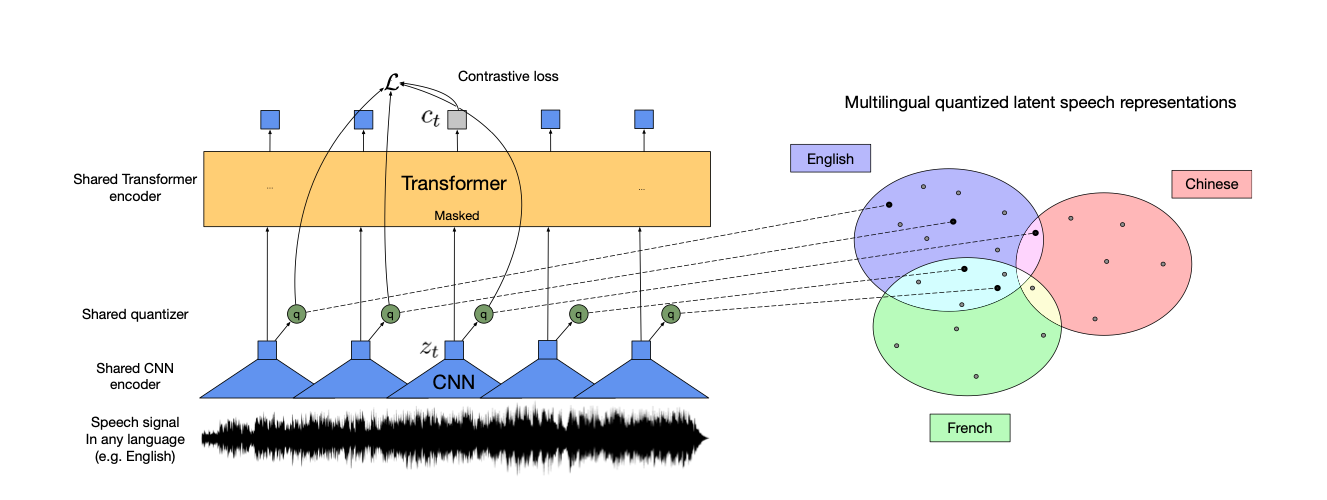
\includegraphics[width=\textwidth]{diagrams/xlsr.png}
    \caption{High level view of the Framework of XLSR \cite{babu_xls-r_2021}.}
    \label{fig:figxlsr}
\end{figure}

\subsection{Feature Extraction}

The feature encoder is a 7-layer, 512 channel CNN that translates a waveform into feature vectors, reducing the dimension of the audio 
to 1D. It does this every 20ms and has a receptive field of 400 samples which is equivalent to 25ms of audio sampled at 16kHz. The feature 
extractor also normalises the audio before it is then forwarded into the network. 


\subsection{Quantisation}
The key challenge of audio related speech data is that it is continuous. Written language can be naturally segmented into words, sentences and subwords while speech does not have 
this natural sub-unit. The quantisation module addresses the continuous nature of speech data, automatically learning discrete speech units such as phonemes and words. It does this through 
sampling from the Gumbel-Softmax distribution, the possible units are comprised of codewords which are grouped in codebooks. The speech unit is the concatenation of these codewords. 
In wav2vec 2.0 there are 2 groups with 320 words in each group and a theoretical maximum of 102400 speech units. The features are multiplied by the quantisation matrix, 
to produce logits and then converting those into probabilities of a codeword matching an exisitng codeword in the codebook using the  Gumbel-Softmax. This module is illustrated in the Figure 
\ref{fig:quantisation}. 

\begin{figure}[h!]
    \centering
    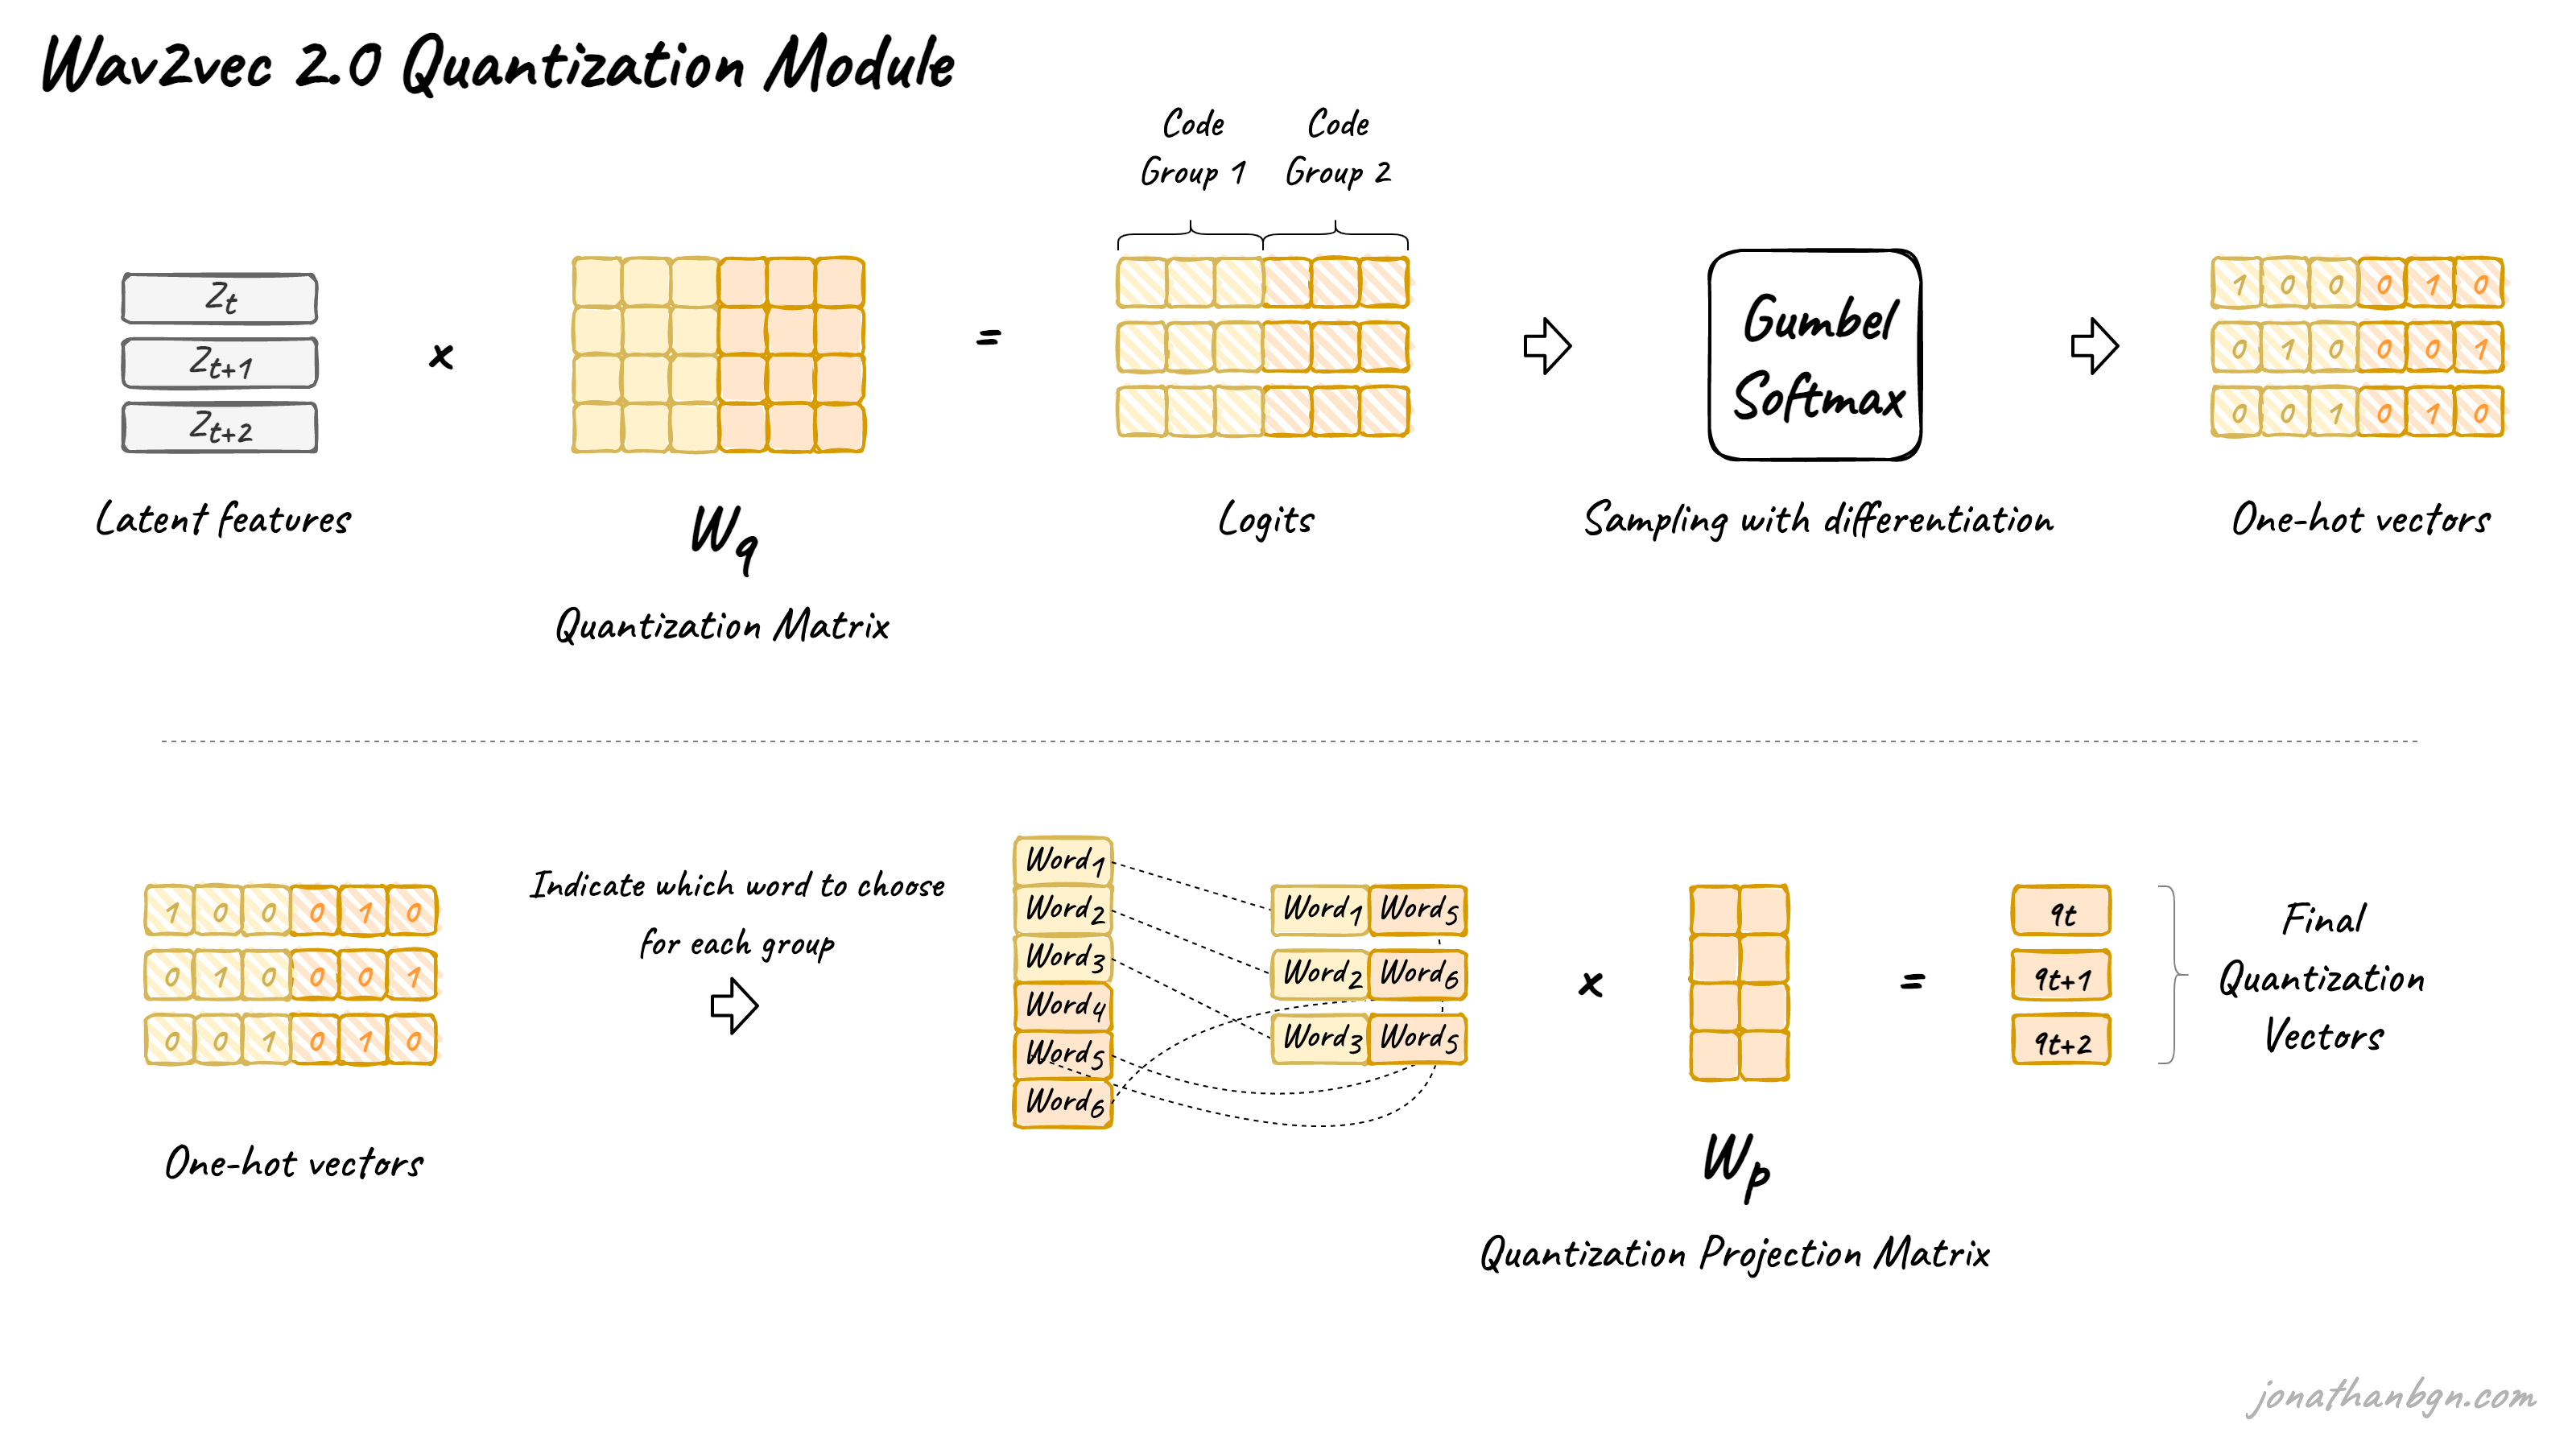
\includegraphics[width=\textwidth]{quantization_module.png}
    \caption{High Level view of the operation of the Quantisation Module \cite{jonathan_bgn_wav2vec2_2021}.}
    \label{fig:quantisation}
\end{figure}


\subsection{Context Network: Transformer Encoder-Decoders}
At the core of wav2vec is a context network comprised of 12 transformer based encoders. The transformers have an attention based 
encoder-decoder architecture, the structure enables all frames of an audio clip to be processed simultaneously. The concept of a transformer based 
network was proposed in the paper "Attention is All You Need" \cite{vaswani_attention_2017} which aimed to iterate upon the design of sequential Recurrent Neural Networks (RNNs) which could 
only process one frame of speech at a time. The architecture and flow of data is illustrated in the Figure \ref{fig:transformer}. 
The outputs of the feature encoder are fed into these transformers and the high dimensional inputs are then converted into inner embeddings. 
Within the encoders and decoders are self attenuation layers which observe multiple words in an input sequence at one time. They identify the most relevant features and words within the frames. Ensuring that these 
portions of the input sequence are given the most weight and focused on. The self attenuation doesn't preserve the ordering of the 
input frame and so a grouped convolutional layer is used to learn the positional embeddings. During training the input, previous predictions and actual value is fed into the decoder to predict the next output. 
After using the input and previous prediction, to generate a prediction it compares it with the correct result. The attention vectors are converted into human interpretable outputs at the feed forward, linear and softmax layers. 

\begin{figure}[h!]
    \centering
    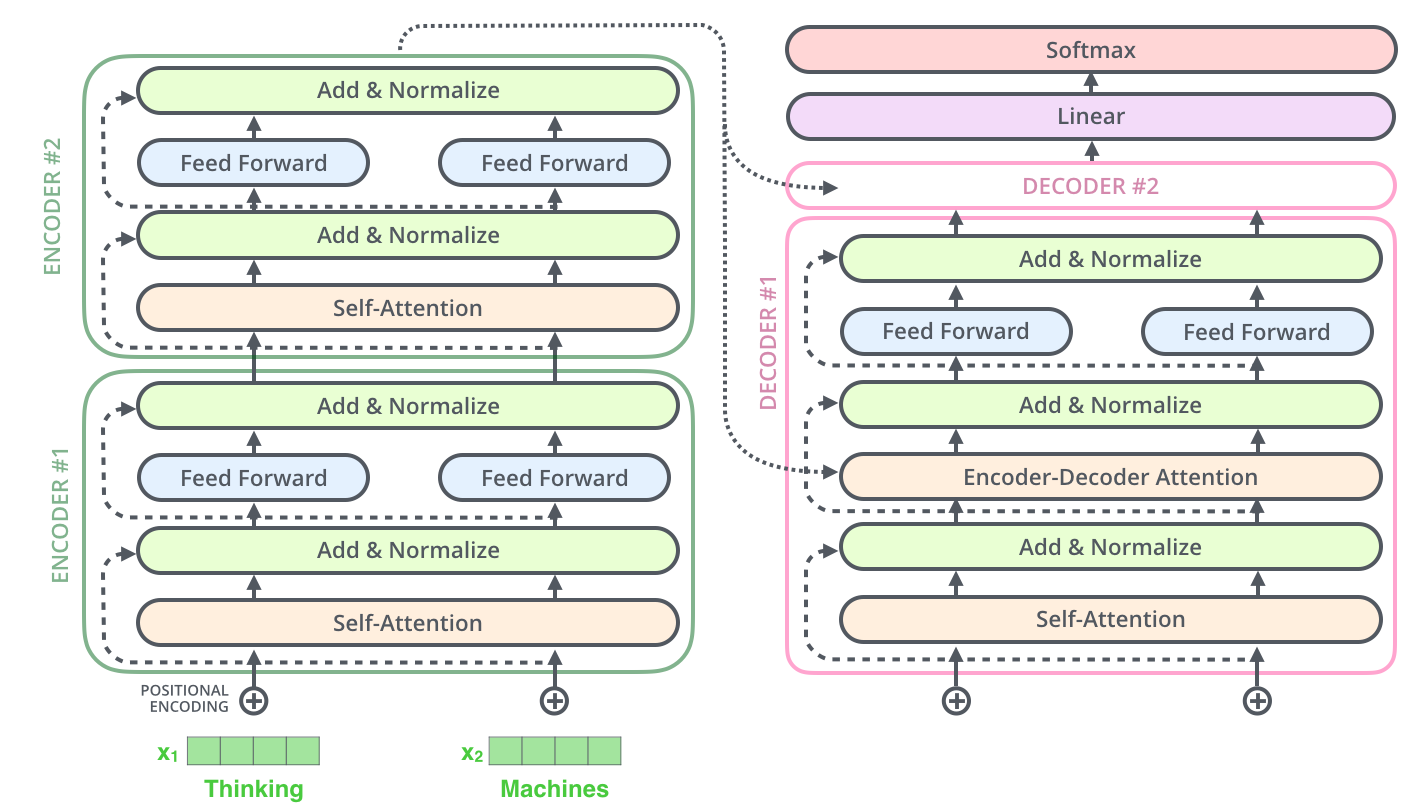
\includegraphics[width=\textwidth]{transformer.png}
    \caption{High Level view of the encoder-decoder transformer \cite{jay_alammar_illustrated_nodate}.}
    \label{fig:transformer}
\end{figure}


Self attention, a key feature of the transformer is defined by the Equation \ref{eqn:selfatten1}. Taking in query $Q$, keys $K$ and values $V$ as the input. 
Their matrices are resulted from multiplying the embeddings' matrix $X$ and their corresponding weight matrices $W_Q$, $W_K$ and $W_V$. 

\[ I = X\times W_I \qquad I \in \{Q,K,V\}\]\label{eqn:selfatten1}

\[attention(Q,K,V) = softmax(Q \cdot K^T)V\]\label{eqn:selfatten2}
\pagebreak
\section{Introduction to Dialectal Arabic}\label{sect:introdialect}
This thesis will focus on Arabic dialects as despite being a widely spoken language and dialects 
being the primary spoken form of Arabic, there are still significant 
improvements that can be made to Arabic DIDs with current systems achieving the highest accuracy of 86.29\%. \\

Arabic is the official language of 25 countries and has 330 million native speakers.
\\Academically the regional dialects are usually grouped into 5 main groups North African (NOR), Egyptian (EGY), Levantine (LEV), Gulf (GLF) and Modern Standard Arabic (MSA). 
MSA is taught academically in most Arabic speaking countries and originates from the Gulf region but is not used 
for general conversation or outside academic setting.

Comparatively to MSA, the lack of standardisation in dialectal Arabic has resulted in more linguist complexities.
Dialectal Arabic has a richer morphology and cliticisation system, accounting for circumfix negation, 
and for attached pronouns to act as indirect objects. As well as this some words are shared but are used for
differing functions eg. For example,'Tyb' is used as an adjective in MSA but dialectal as an interjection. 
North African has the largest amount of dialectical variation within the dialect and is the most different from the other Arabic dialects. Taking influences from French and Berber languages. 
Egyptian globally is the widely understood dialect due to the Egyptian movie and television industry. 
Levantine dialects differ slightly in pronunciation and intonation but are equivalent when transcribed. Closely related to Aramaic. 
Gulf is the form which is most closely related to MSA and preserves many of MSA verb conjugations. 
Understanding of different dialects depends on an individuals exposure outside their own country. eg. due to the prevalence of Egyptian television and movies,
many Arab people can understand the Egyptian Dialect but a Levantine speaker would not be able to understand 
the Moroccan dialect. 

The differences between Arabic dialects are comparable to the differences present in North Germanic languages such as
Norwegian, Swedish, Danish or the West Salvic languages eg. Czech, Slovak, Polish. Some linguistic variation between dialectal Arabic include incongruous morphemes, prepositions
verb conjugations, word meanings, phonemes and pronunciation. Some examples of this is shown in the Table \ref{tab:dialectDifferences}. \cite{biadsy_spoken_2009, boril_arabic_2012}\\

In addition to this, the majority of available pretrained models that are used in self supervised or semi supervised systems are trained on 
English datasets. Arabic has 6 vowels/diphthongs in MSA and 8-10 vowels in most dialects, 
28 constants while English has 24 consonants and 22 vowels. \cite{zaidan_arabic_2014}
As well as this compared to English, Arabic and particularly dialectal Arabic has large amount of morphemes, rendering 
it unfeasible for the training data to contain all the possible morphemes. So, a system which has been built to operate
well for a DID that is linguistically different to English should thereby be robust enough to be applied to other languages with similar complexity.\\ 
Hence, the two key challenges in creating an Arabic DID which will be explored in this thesis are: 
\begin{itemize}
    \item Dialectal Arabic is considered low resource, as there are no large commercially available datasets. 
    \item There is a significant amount of complex linguist differences and similarities between Arabic dialects. 
\end{itemize}
More details about the ADI17 dataset to be used is provided in Section \ref{sect:dataset}, 
the dataset contains audio from 17 countries and be divided into the 4 widely spoken major dialect groups (NOR, EGY, LEV, GLF), 
as MSA is not spoken in general conversation it is not included in the dataset and will not be identified by the DID designed in this thesis.\\
\begin{table}[htb]
    \begin{center}
    \begin{tabular}{|c || c | c | c | c|}
    \hline
    English/Feature & MSA & LEV & GLF & EGY \\ [0.5ex] 
    \hline\hline
    Money & nqwd & mSAry & flws & flws \\ 
    \hline
    I want & Aryd & bdy & Ab\textgammaý & ςAyz \\
    \hline
    Now & AlĀn & hlq & AlHyn & dlwqt \\
    \hline
    When? & mtý? & Aymtý? & mtý? & Amtý \\
    \hline
    alveolar affricate sound & dj & j & y & g \\
    \hline
    Handsome & djami:l & jami:l & yami:l & gami:l \\
    \hline
    consonant sound & \textTheta & t & \textTheta & t \\
    \hline
    Three & {\textTheta}ala:{\textTheta}a & tla:te  & {\textTheta}ala:{\textTheta}a  & tala:ta \\[0.5ex] 
    \hline
    \end{tabular}
    \caption{Examples of linguistic differences between Arabic Dialects}
    \label{tab:dialectDifferences}
    \end{center}
\end{table}